\documentclass[11pt,a4paper]{article}

\usepackage{style2017}
\usepackage{hyperref}
\usepackage{pifont}
\hypersetup{
    colorlinks =false,
    linkcolor=blue,
   linkbordercolor = 1 0 0
}
\newcounter{numexo}
\setcellgapes{1pt}

\newcommand{\nd}{n\oe{}ud~}
\newcommand{\Nd}{N\oe{}ud~}
\newcommand{\nds}{n\oe{}uds~}

\setlength{\parskip}{0.5em}

\lstset{%
	language={python},
	frame=single,
	xleftmargin=2cm,
	xrightmargin=2cm,
	basicstyle = \ttfamily,
	breaklines=true,
	%numbers=left,
	numberstyle=\footnotesize,
	captionpos=b,
	basicstyle=\ttfamily,
	keywordstyle=\bfseries\color{blue},
	commentstyle=\itshape\color{green},
	moredelim=[il][\color{red}]{/+},%
	}
	
\begin{document}



\begin{NSI}
{Activité}{Algorithme glouton}
\end{NSI}


\subsection*{Problème du rendue de monnaie}

Le système monétaire européen basé sur l'euro utilise des pièces de 1 et 2 euros et des billets de 5, 10, 20, 50, 100 et 200 euros. Il est possible avec ce système monétaire de réaliser toutes les sommes entières en supposant qu'on ait suffisamment de pièces et de billets.

On suppose dans cette activité que l'on a des pièces et billets en \textbf{quantité infinie} parmi les valeurs 1, 2, 5, 10, 20, 50, 100 et 200 euros.

\begin{enumerate}
\item On doit rendre 9 euros à une personne.
\begin{enumerate}
\item Combien existe-t-il de manières différentes pour réaliser cette somme ?
\item Quelle est la combinaison qui utilise le moins de pièces et billets ?
\end{enumerate}
\item Comment rendre avec le moins de pièces et billets possible la somme de 27 euros ?


\item On cherche à réaliser une somme en utilisant le moins de pièces et de billets possible. Une stratégie pour déterminer la meilleure solution consiste à soustraire à la somme à rendre les plus grosses valeurs de pièces ou de billets jusqu'à obtenir 0 euro. Cette stratégie est dite \textbf{gloutonne}.

\begin{enumerate}
\item Vérifier qu'elle convient pour la somme à rendre de 27 euros.
\item Appliquer cette stratégie pour rendre la somme de 48 euros.
\end{enumerate}

\item On remplace le système monétaire européen par un système où les unités monétaires ont pour valeurs 1, 3, 6, 12, 24 et 30.
\begin{enumerate}
\item Comment rendre la somme de 27 euros de manière optimisée?
\item Comment rendre la somme de 48 euros de manière optimisée?
\item Est-ce que la stratégie gloutonne répond correctement au problème pour ces deux sommes ?
\end{enumerate}
\item Quelle conclusion peut-on donner sur l'algorithme glouton utilisé dans ce problème d'optimisation ?
\end{enumerate}


\subsection*{Programmation python}

On donne, en langage naturel, l'algorithme glouton du rendu de monnaie:

\begin{lstlisting}
nombre pièces = 0
pour chaque pièce du système monétaire:
	tant que somme à rendre > pièce:
		nombre pièces = nombre pièces + 1
		somme à rendre = somme à rendre - pièce
\end{lstlisting}

\begin{enumerate}
\item Créer un tableau \textsf{systeme\_monetaire} en Python contenant les unités (pièces et billets) du système monétaire utilisé.

\item Écrire une fonction \textsf{rendu\_monnaie} qui prend en paramètre la somme à rendre et renvoie le nombre de pièces et billets pour réaliser la somme à rendre. 

\item Écrire une variante de la fonction \textsf{rendu\_monnaie} qui prend en paramètre la somme à rendre et renvoie sous forme de liste les pièces à rendre pour réaliser la somme. 

%\item Modifier vos fonctions pour qu'elles prennent en paramètre les valeurs monétaires utilisées.

\item Écrire une version récursive de la fonction \textsf{rendu\_monnaie}.
\end{enumerate}

%\subsection*{Recherche de la meilleure solution}
%L'objectif est de mettre en place, si possible, un algorithme qui donne la meilleure solution au problème.
%
%On donne l'algorithme en python suivant:
%\begin{center}
%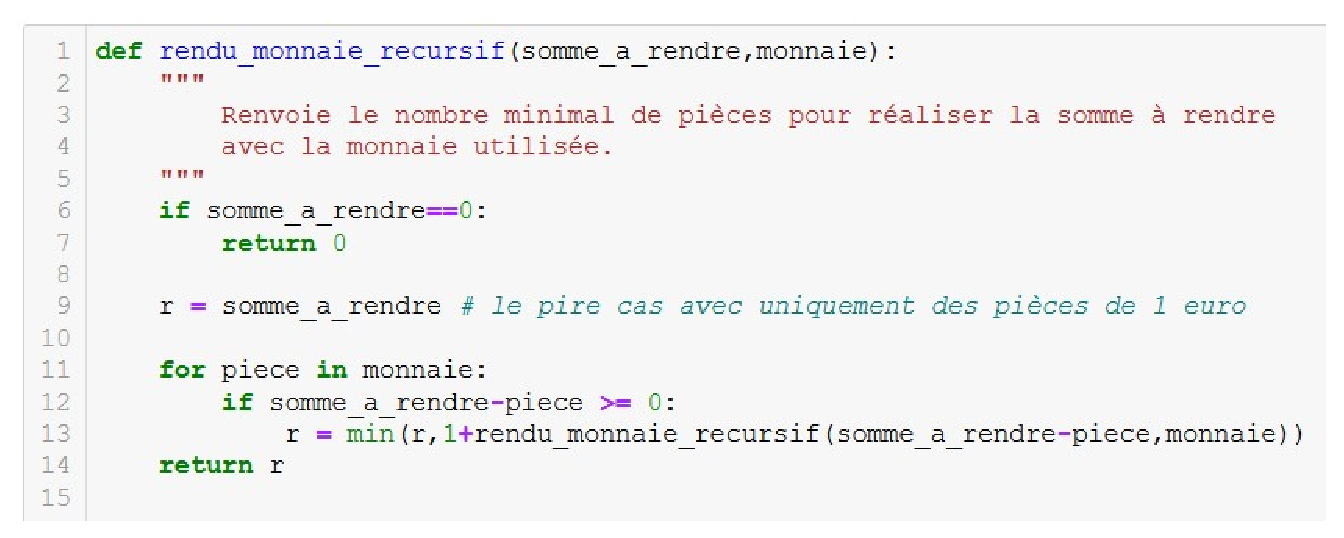
\includegraphics[scale=0.8]{img/act-1.eps}
%\end{center}
%
%\begin{enumerate}
%\item Programmer cet algorithme puis l'appliquer avec les exemples précédents.
%\item On réduit la monnaie aux deux pièces de 1 et 2 euros.
%\begin{enumerate}
%\item Appliquer cet algorithme pour rendre la somme de 30. Puis avec 35 euros.
%\item Déterminer le nombre d'appels récursifs pour rendre 3 euros.
%\item Déterminer le nombre d'appels récursifs pour rendre 4 euros.
%\item Déterminer le nombre d'appels récursifs pour rendre 5 euros.
%\item Déterminer le nombre d'appels récursifs pour rendre 6 euros.
%\item Déterminer le nombre d'appels récursifs pour rendre 7 euros.
%\end{enumerate} 
%\item Faire une recherche sur la suite de Fibonacci et établir un lien avec la question précédente.
%\end{enumerate}
%
%
%
%\subsection*{Programmation dynamique}
%
%L'algorithme précédent renvoie la meilleure solution mais ne permet pas de le faire pour des valeurs très élevées.
%
%Pour rendre cet algorithme plus efficace, on a recourt à la programmation dynamique.
%
%\begin{enumerate}
%\item \textbf{Phase 1:} Recherche documentaire
%
%Sur wikipédia : attention, les contenus sont assez difficiles et sont parfois hors programme comme la mémoïsation
%\begin{enumerate}
%\item Problème du rendu de monnaie
%\item Programmation dynamique
%\end{enumerate}
%Sur le site Pixees de David Roche : programmation dynamique
%
%\item \textbf{Phase 2:} Programmation
%
%Écrire en python, un algorithme qui donne la meilleure solution au problème du rendu de monnaie avec la programmation dynamique.
%
%\item \textbf{Phase 3:} Rédaction
%
%Rédiger un document qui présente le problème du rendu de monnaie, les différentes approches algorithmiques possibles et des applications qui reposent sur ce problème.
%\end{enumerate}

\end{document}
